\documentclass[a4paper,12pt]{article}
\usepackage[english]{babel}
\usepackage[utf8]{inputenc}
\usepackage{amsmath}
\usepackage{amsthm}
\usepackage{amsfonts}
\usepackage{amssymb}
\usepackage{graphicx}
\usepackage{hyperref}
\usepackage{enumitem}
\usepackage{float}
\usepackage{booktabs}
\usepackage{xcolor}
\usepackage{algorithm}
\usepackage{algpseudocode}
\usepackage{CJKutf8}
\usepackage[colorinlistoftodos]{todonotes}
\usepackage[left=1.50cm, right=1.50cm, top=1.20cm]{geometry}
\usepackage{listings}
\usepackage{tikz}
\usetikzlibrary{positioning,arrows,calc}
\tikzset{
modal/.style={>=stealth',shorten >=1pt,shorten <=1pt,auto,node distance=1.5cm,semithick},
world/.style={circle,draw,minimum size=0.5cm,fill=gray!15},
point/.style={circle,draw,inner sep=0.5mm,fill=black},
reflexive above/.style={->,loop,looseness=7,in=120,out=60},
reflexive below/.style={->,loop,looseness=7,in=240,out=300},
reflexive left/.style={->,loop,looseness=7,in=150,out=210},
reflexive right/.style={->,loop,looseness=7,in=30,out=330}
}

\linespread{1.5}

\title{LeetCode 1 --- 30}
\author{SS}

\begin{document}
\maketitle

\section{2 -- Add Two Numbers}
You are given two non-empty linked lists $L_1$ and $L_2$ representing two non-negative integers. The digits are stored in reverse order and each of their nodes contain a single digit. Add the two numbers and return it as a linked list.
\par
You may assume the two numbers do not contain any leading zero, except the number 0 itself.
\paragraph{Example:}
\begin{flushleft}
\textbf{Input}:
\begin{figure}[H]
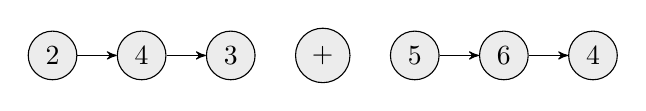
\begin{tikzpicture}
[mynode/.style={circle, draw, minimum size=2mm, fill=gray!15}]
\node(){};
\node(2) [mynode] {2};
\node(4) [mynode, right=5mm of 2] {4};
\node(3) [mynode, right=5mm of 4] {3};
\node(a) [mynode, right=5mm of 3] {$+$};
\node(5) [mynode, right=5mm of a] {5};
\node(6) [mynode, right=5mm of 5] {6};
\node(41) [mynode, right=5mm of 6] {4};
\draw[->,>=stealth'] (2)--(4);
\draw[->,>=stealth'] (4)--(3);
\draw[->,>=stealth'] (5)--(6);
\draw[->,>=stealth'] (6)--(41);
\end{tikzpicture}
\end{figure}
\textbf{Output}
\begin{figure}[H]
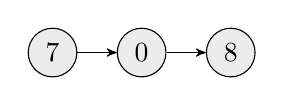
\begin{tikzpicture}
[mynode/.style={circle, draw, minimum size=2mm, fill=gray!15}]
\node(){};
\node(7) [mynode] {7};
\node(0) [mynode, right=5mm of 7] {0};
\node(8) [mynode, right=5mm of 0] {8};
\draw[->,>=stealth'] (7)--(0);
\draw[->,>=stealth'] (0)--(8);
\end{tikzpicture}
\end{figure}
\textbf{Explanation}: $342 + 465 = 807$.
\end{flushleft}


\section{3 --  Longest Substring Without Repeating Characters}
Given a string $S$, find the length of the longest substring without repeating characters.
\paragraph{Example 1:}
\begin{flushleft}
\textbf{Input}: \texttt{abcabcbb}
\\
\textbf{Output}: 3 
\\
\textbf{Explanation}: The answer is \texttt{abc}, with the length of 3. 
\end{flushleft}
\paragraph{Example 2:}
\begin{flushleft}
\textbf{Input}: \texttt{bbbbb}
\\
\textbf{Output}: 1
\\
\textbf{Explanation}: The answer is \texttt{b}, with the length of 1.
\end{flushleft}
\paragraph{Example 3:}
\begin{flushleft}
\textbf{Input}: \texttt{pwwkew}
\\
\textbf{Output}: 3
\\
\textbf{Explanation}: The answer is \texttt{wke}, with the length of 3. Note that the answer must be a substring, \texttt{pwke} is a subsequence and not a substring.
\end{flushleft}
\subsection{Hash Map Approach}
\begin{CJK*}{UTF8}{gbsn}
用一个\texttt{hashmap}来记录每个字符出现的位置,并逐步更新最新的位置。这是因为如果字符$s[j]$在$s[\alpha\ldots j-1]$中在$k$处重复,那么只需要把$\alpha$更新到$k+1$就可以了。
\end{CJK*}
\subsubsection{Code}
Procedure \texttt{GetLongestSubstring} returns the longest slide window for input string $S$.
\begin{algorithm}[H]
\caption{Get longest substring without duplicates}
\begin{algorithmic}[1]
\Procedure{GetLongestSubstring}{$S$}
\State $M$ as $M[0]=\ldots=M[255]:=-1$.
\State $\alpha := 0 $
\State $\beta := 0$ \Comment The maximum length so far
\For{$i := 0$ \textbf{to} $|S|$}
\If{$M(S(i)) \neq -1$} \Comment found repeat $S(i)$ in $S(\alpha\ldots i-1)$
\State $\alpha \gets \max(\alpha, M(S(i))) + 1$ \Comment update to the next index of the duplicate
\EndIf
\State $\beta \gets \max(\beta, i - \alpha +1 )$ \Comment update maximum length so far
\State $M(S(i)) \gets i$ \Comment update $S(i)$ latest index
\EndFor
\State \Return $\beta$
\EndProcedure
\end{algorithmic}
\end{algorithm}

\section{4 --- Median of Two Sorted Arrays}
There are two sorted arrays $A$ and $B$ of size $m$ and $n$ respectively.
\par
Find the median of the two sorted arrays. The overall run time complexity should be $O(\log (m+n))$.
\par
You may assume $A$ and $B$ cannot be both empty.
\paragraph{Example 1:}
\begin{flushleft}
\textbf{Input}: $A = [1, 3]$, $B = [2]$
\\
The median is 2.0
\end{flushleft}
\paragraph{Example 2:}
\begin{flushleft}
\textbf{Input}: $A = [1, 2]$, $B = [3, 4]$
\\
The median is $(2 + 3)/2 = 2.5$
\end{flushleft}
\subsection{Binary Search Approach}
\textbf{\large{Note:}}
\par
\vspace{0.5em}
\begin{CJK*}{UTF8}{gbsn}
\begin{itemize}
\item 假设数组$A$和$B$中,$A[P_A-1]$个和$B[P_B-1]$是处于两个数组合并后处于\texttt{median}处的元素,无论$L_A+L_B$是否为奇偶数,合并后的数组处于$A[P_A-1]$和$B[P_B-1]$之前的元素个数必然是$(L_A+L_B-1)/2$,例如如果$L_A+L_B = 9$,那么\texttt{median}左右的元素个数为$(L_A+L_B-1)/2=4$,因为这时候\texttt{median} 只有一个元素。如果$L_A+L_B = 10$,那么这时候\texttt{median}有两个元素,但是这两个元素的左右两边的元素个数仍然为$(L_A+L_B-1)/2=4$,不同的只是这时候\texttt{median}是两个元素。至于$A[P_A-1]$和$B[P_B-1]$谁是\texttt{median}还是两者都是,没有关系。
\item 根据上述分析,就可以得到$P_A-1+P_B-1 =(L_A+L_B-1)/2 $,变换一下形式,得到如下关系
\[
P_A + P_B = (L_A+L_B+1)/2
\]
\item 采用二分法查询在数组A中的$P_A$位置,使得上述关系成立,同时还需要有以下关系
\[
A[P_A - 1] \leq B[P_B] \quad \mathtt{and} \quad B[P_B - 1] \leq A[P_A]
\]
这是因为$A[P_A-1]$个和$B[P_B-1]$是处于两个数组合并后处于\texttt{median}处的元素,如果不能满足以上关系,$A[P_A-1]$个或者$B[P_B-1]$就不再是处于\texttt{median}处的元素了。
\item 由于$P_A$的取值范围是$0\to L_A$,所以$P_B$的取值范围就是$(L_B-L_A+1)/2 \to (L_A+L_B+1)/2$。为了保证$P_B$的最小值仍然大于等于0,可以强制设定$L_B$为$A$, $B$中的较长数组。
\end{itemize}
\end{CJK*}
\subsubsection{Code}
Procedure \texttt{FindMedian} returns the median value of $A$ and $B$ with size $m$ and $n$ respectively.
\setcounter{algorithm}{0}
\begin{algorithm}[H]
\caption{Binary Search Approach}
\begin{algorithmic}[1]
\Procedure{FindMedian}{$A, m, B, n$}
\State $\ell: = (m + n + 1)/2$ \Comment set half length for the merged array
\If{$m > n$}
\State \textbf{swap} $A$ and $B$ \Comment make sure $B$ is the \textbf{longer} array
\EndIf
\State $l := 0$ and $r:=m$ \Comment Start binary search
\While{$l \leq r$}
\State $P_A := (l+r)/2$ \Comment get middle point in $A$
\State $P_B := \ell - P_A$ \Comment get number of elements need to be from $B$
\If{$P_A > 0 $ \textbf{and} $A[P_A-1] > B[P_B]$ }
\State $r \gets P_A -1 $ \Comment Search in the lower half
\ElsIf{$P_A < L_A $ \textbf{and} $ A[P_A] < B[P_B-1]$}
\State $l \gets P_A +1 $ \Comment Search in the upper half
\Else
\If{$P_A=0$}
\State $\theta_1 := B[P_B-1]$ \Comment No element from $A$ below than \textbf{median}
\ElsIf{$P_B = 0$}
\State $\theta_1 := A[P_A-1]$ \Comment No element from $B$ below than \textbf{median}
\Else 
\State $\theta_1 := \max(A[P_A - 1], B[P_B-1])$ \Comment The lower median is the greater one
\EndIf
\If{$P_A = m$}
\State $\theta_2 := B[P_B]$ \Comment all elements from $A$ below than \textbf{median}
\ElsIf{$P_B = n$}
\State $\theta_2 := A[P_A]$ \Comment all elements from $B$ below than \textbf{median}
\Else
\algstore{myalg}
\end{algorithmic}
\end{algorithm}

\begin{algorithm}[H]
\begin{algorithmic}[1]
\algrestore{myalg}
\State $\theta_2 := \min(A[P_A], B[P_B])$ \Comment The lower median is the \textbf{smaller} one
\EndIf
\EndIf
\If{$(m+n) \bmod 2 = 0$} \Comment even length
\State \Return $(\theta_1 + \theta_2)/2$
\Else \Comment odd length
\State \Return $\theta_1$
\EndIf
\EndWhile
\EndProcedure
\end{algorithmic}
\end{algorithm}

\section{5 -- Longest Palindromic Substring}
Given a string $S$, find the longest palindromic substring in $S$. You may assume that the maximum length of $s$ is 1000.
\paragraph{Example 1:}
\begin{flushleft}
\textbf{Input}: \texttt{babad}
\\
\textbf{Output}: \texttt{bab}
\\
\textbf{Note}:  \texttt{aba} is also a valid answer.
\end{flushleft}
\paragraph{Example 2:}
\begin{flushleft}
\textbf{Input}: \texttt{cbbd}
\\
\textbf{Output}: \texttt{bb}
\end{flushleft}
\subsection{Dynamic Programming Approach}
\begin{CJK*}{UTF8}{gbsn}
方法一: \texttt{Dynamic Programming}. \texttt{DP}方法也有两种,以长度为循环条件,以及倒序推。两种方法的\texttt{DP}公式一样
\[
DP[i][j]  = 
\begin{cases}
 0 & \iff S[i] \neq S[j] \\
 DP[i+1][j-1] &\iff S[i] = S[j]
\end{cases}
\]
\par
这两种\texttt{DP}所需的空间复杂度都为$O(n^2)$,但是第二种方法可以做进一步修改,使得空间复杂度为$O(n)$
\par
方法二: 由于只有一维数组,所以数组中的每个元素在循环中都要被更新而不是固定不变,这点是和二维\texttt{DP}不同的地方。
\end{CJK*}
\subsubsection{Code}
Procedure \texttt{LongestPalindrome} returns the longest palindrome string for input string $S$.
\setcounter{algorithm}{0}
\begin{algorithm}[H]
\caption{\texttt{DP} Method 1: loop by substring length}
\begin{algorithmic}[1]
\Procedure{LongestPalindrome}{$S$}
\State \texttt{DP} := \textbf{boolean array} with $|S|\times|S|$
\State $L_\mathtt{max} := 1$ \Comment maximum palindrome length is initialized with \textbf{1} 
\For{$i:=0$ \textbf{to} $|S|-1$}
\State $\mathtt{DP}[i][i] \gets 1$ \Comment single character is \textbf{palindrome} by itself.
\EndFor
\For{$l:=2$ \textbf{to} $|S|$} \Comment substring length from $2 \to |S|$
\For{$i := 0$ \textbf{to} $|S| - l$} \Comment the start of substring is from $0 \to |S| - l$
\State $j := i + l - 1$ \Comment the end of substring
\If{$S[i] \neq S[j]$}
\State $\mathtt{DP}[i][j] = 0$ \Comment $S[i\ldots j] $cannot be \textbf{palindrome}
\Else
\State $\mathtt{DP}[i][j] = \mathtt{DP}[i+1][j-1]$ 
\EndIf
\If{$\mathtt{DP}[i][j] = \mathtt{true}$} \Comment $S[i\ldots j]$ is \textbf{palindrome}
\If{$L_\mathtt{max} < l$}
\State $S_\mathtt{max} := S[i\ldots j]$ \Comment update \textbf{longest palindrome} as $S[i\ldots j]$
\State $L_\mathtt{max} \gets l$ \Comment update \textbf{maximum palindrome length}
\EndIf
\EndIf
\EndFor
\EndFor
\State \Return $S_\mathtt{max}$
\EndProcedure
\end{algorithmic}
\end{algorithm}

\begin{algorithm}[H]
\caption{\texttt{DP} Method 2: backward}
\begin{algorithmic}[1]
\Procedure{LongestPalindrome}{$S$}
\State \texttt{DP} := \textbf{1 dimension array} with $\mathtt{size} = |S|$ and all elements are \textbf{false}
\State $L_\mathtt{max} := 1$ \Comment maximum palindrome length is initialized with \textbf{1} 
\For{$i:=|S|-1$ \textbf{to} $0$}
\For{$j:=|S|-1$ \textbf{to} $i$}
\If{$S[i] \neq S[j]$}
\State $\mathtt{DP}[j] \gets \mathtt{false}$ \Comment Update $\mathtt{DP}[j]$ in each loop although it is \textbf{true} in previous loop
\Else
\If{$j-i\leq 2$}
\State $\mathtt{DP}[j] \gets \mathtt{true}$ \Comment If substring length $\leq 2$, directly update $\mathtt{DP}[j]$
\Else 
\State $\mathtt{DP}[j] \gets \mathtt{DP}[j-1]$ \Comment  Update $\mathtt{DP}[j]$ as $\mathtt{DP}[j-1]$ 
\EndIf
\EndIf
\If{$\mathtt{DP}[j] = \mathtt{true}$} \Comment Found palindrome
\If{$j-i +1 > L_\mathtt{max}$} \Comment Found maximum palindrome so far
\State $L_\mathtt{max} \gets j-i +1$
\State $S_\mathtt{max} \gets S[i\ldots j]$
\EndIf
\EndIf
\EndFor
\EndFor
\State \Return $S_\mathtt{max}$
\EndProcedure
\end{algorithmic}
\end{algorithm}


\section{6 --- ZigZag Conversion}
The string \texttt{PAYPALISHIRING} is written in a zigzag pattern on a given number of rows like this: 
\\
P\hspace{1.5em}A\hspace{1.5em}H\hspace{1.5em}N
\\
A\hspace{0.5em}P\hspace{0.5em}L\hspace{0.5em}S\hspace{0.5em}I\hspace{0.5em}I\hspace{0.5em}G
\\
Y\hspace{1em}I\hspace{1em}R
\\
And then read line by line: \texttt{PAHNAPLSIIGYIR}
\par
Write the code that will take a string and make this conversion given a number of rows:

\textbf{\large{Note:}}
\par
\vspace{0.5em}
\noindent
\textbf{Approach 1:}
\par
\noindent
Visit all characters in row 0 first, then row 1, then row 2, and so on\dots
\par
\noindent
Denote number of rows as $N$
\begin{itemize}
\item Characters in row $0$ are located at indexes $0, \left(2 \times N - 2\right), 2\times\left(2 \times N - 2\right), \ldots$
\item Characters in row $N-1$ are located at indexes $N-1, \left(2 \times N - 2\right) + N - 1, 2\times\left(2 \times N - 2\right) + N - 1, \ldots$
\item Characters in inner row $0<i<N-1$ are located at indexes 
\[
i, \left(2 \times N - 2\right)-i, \left(2 \times N - 2\right) + i, 2\times\left(2 \times N - 2\right)- i, 2\times\left(2 \times N - 2\right)+ i, 3\times\left(2 \times N - 2\right)- i, \dots
\]
\end{itemize}
\setcounter{algorithm}{0}
\begin{algorithm}[H]
\caption{Print letters in Zigzag way}
\begin{algorithmic}[1]
\Statex
\Procedure{Zigzag}{$S$, $N$}
\If{$N = 1$}
\State \Return $S$ \Comment one row is $S$ itself
\EndIf
\State $\mathtt{STEP} := 2 \times N -2$
\State $Z:= \emptyset$ \Comment $Z$ will be the print string
\For{$n:=0$ \textbf{to} $N-1$}
\State $k:= 0$
\While{$k+n < L_{S}$}
\State $Z \gets Z + S[k+n]$ \Comment $S[m\times \left(2 \times N - 2\right)] + i$ for $m = 1,2, \ldots$ and $i = 0, \ldots, N-1$
\If{$n\neq 0$ \textbf{and} $n\neq N-1$ \textbf{and} $k+\mathtt{STEP} - n < L_{S}$} \Comment For inner rows
\State $Z \gets Z + S[k+\mathtt{STEP}-n]$ \Comment get $S[m\times\left(2 \times N - 2\right)- i]$
\EndIf
\State $k \gets k+\mathtt{STEP}$
\EndWhile
\EndFor
\State \Return $Z$
\EndProcedure
\Statex
\end{algorithmic}
\end{algorithm}

\section{7 --- Reverse Integer}
Given a 32-bit signed integer $N$, reverse digits of an integer.
\paragraph{Example 1:}
\begin{flushleft}
\textbf{Input}: 123
\\
\textbf{Output}: 321
\end{flushleft}
\paragraph{Example 2:}
\begin{flushleft}
\textbf{Input}: $-123$
\\
\textbf{Output}: $-321$
\end{flushleft}
\paragraph{Example 3:}
\begin{flushleft}
\textbf{Input}: 120
\\
\textbf{Output}: 21
\end{flushleft}
\paragraph{Note:}
Assume we are dealing with an environment which could only store integers within the 32-bit signed integer range: $[-2^{31}, 2^{31}-1]$. For the purpose of this problem, assume that your function returns 0 when the reversed integer overflows.
\subsection{Intuition}
We can build up the reverse integer one digit at a time. While doing so, we can check beforehand whether or not appending another digit would cause overflow.
\begin{itemize}
\item Reversing an integer can be done similarly to reversing a string.
\item We want to repeatedly \textbf{pop} the last digit off of $x$ and \textbf{push} it to the back of the $\mathbf{R}$. In the end, $\mathbf{R}$ will be the reverse of the $x$.
\item To \textbf{pop} and \textbf{push} digits without the help of some auxiliary stack/array
\begin{itemize}
\item \textbf{pop}: 

\begin{align*}
\mathtt{pop} &= x \bmod 10 \\
x &= \frac{x}{10}
\end{align*}

\item \textbf{push}:
\begin{align*}
T &= R \times 10 + \mathtt{pop} \\
R &= T
\end{align*}
\end{itemize}
\item However, $T$ could be overflow, Suppose $I_{\max}$ is the maximum value represented by integer type.
\begin{enumerate}
\item if $T = R \times 10 + \mathtt{pop}$ has overflow, it must be $R \geq \dfrac{I_{\max}}{10}$
\item if $R > \dfrac{I_{\max}}{10} $, $T$ will be overflow for sure.
\item if $R = \dfrac{I_{\max}}{10}$, $T$ will be overflow $\iff \mathtt{pop} > 7$, because $I_{\max} = 2^{31} - 1 = 2147483647$
\end{enumerate}
\item similar when $R$ is underflow, and $I_{\min} = -2^{31} = -2147483648$
\end{itemize}

\setcounter{algorithm}{0}
\begin{algorithm}[H]
\caption{Reverse an integer}
\begin{algorithmic}[1]
\Statex
\Procedure{ReverseInteger}{$N$}
\State $R:=0$ \Comment $R$ is the result of reverse
\State $R_{\max}:= \dfrac{I_{\max}}{10}$ \Comment threshold for $R$ to avoid overflow
\State $R_{\min}:= \dfrac{I_{\min}}{10}$ \Comment threshold for $R$ to avoid underflow
\While{$N \neq 0$}
\State $\mathtt{pop} := N \bmod 10$
\State $N = \dfrac{N}{10}$
\If{$R > R_{\max}$ \textbf{or} ($R=R_{\max}$ \textbf{and} $\mathtt{pop} > 7$)} \Comment overflow
\State \Return 0
\ElsIf{$R < R_{\min}$ \textbf{or} ($R=R_{\min}$ \textbf{and} $\mathtt{pop} < -8$)} \Comment underflow
\State \Return 0
\Else
\State $R\gets R\times 10 + \mathtt{pop}$
\EndIf
\EndWhile
\EndProcedure
\Statex
\end{algorithmic}
\end{algorithm}

\section{9 --- Palindrome Number}
\textbf{\large{Note:}}
\par
\noindent
\paragraph{Intuition}
\begin{itemize}
\item The first idea that comes to mind is to convert the number into string, and check if the string is a palindrome, but this would require extra non-constant space for creating the string which is not allowed by the problem description.
\item Second idea would be reverting the number itself, and then compare the number with original number, if they are the same, then the number is a palindrome. However, if the reversed number is larger than $2^{32}$, it causes integer overflow.
\item Following the thoughts based on the second idea, to avoid the overflow issue of the reverted number, what if revert {\color{red}half} of the number? After all, the reverse of the last half of the palindrome should be the same as the first half of the number, if the number is a palindrome.
\par
For example, if the input is 1221, if we can revert the last part of the number \textbf{1221} from {\textbf{\color{blue}21}} to {\textbf{\color{red}12}}, and compare it with the first half of the number \textbf{12}, since 12 is the same as 12, we know that the number is a palindrome.
\end{itemize}
\paragraph{Algorithm}
\begin{itemize}
\item All {\color{red}negative} numbers are not palindrome, for example: $-123$ is not a palindrome since the $-$ does not equal to $3$. 
\item All multiply of \textbf{10} are not palindrome. The first number cannot be {\color{red}0}
\item How to know reaching the {\color{red}half} of the number? Since the number is divided by 10, and the reversed number is multiplied by 10, when the original number is {\color{red}less than} the reversed number, it means we've processed half of the number digits.
\item If the number length is odd, such as \textbf{12321}. When loop ended, the reversed number will be $12$, while origin number becomes $123$. Therefore, need to check if $12 = \dfrac{123}{10}$
\end{itemize}
\setcounter{algorithm}{0}
\begin{algorithm}[H]
\caption{Check if the integer is a palindrome number}
\begin{algorithmic}[1]
\Statex
\Procedure{IsPalindrome}{$N$}
\If{$N < 0$ \textbf{or} $N \bmod 10 \equiv 0$} \Comment {{\color{red}negative}} or multiply of \textbf{10} cannot be palindrome number
\State \Return \textbf{false} 
\EndIf
\State \textbf{$R := 0$} \Comment $R$ is the \textbf{reversed number}
\While{$N > R$} \Comment check if reaching to half of $N$
\State $q := N\div 10$
\State $r := N\bmod 10$
\State $R \gets R\times 10 + r$
\State $N\gets q$ \Comment Update $N$
\EndWhile
\If{$N \neq R$ \textbf{and} $N \neq \dfrac{R}{10}$} \Comment {{\color{red}cannot}} be palindrome number
\State \Return \textbf{False}
\Else
\State \Return \textbf{True}
\EndIf
\EndProcedure
\Statex
\end{algorithmic}
\end{algorithm}

\section{10 --- Regular Expression Matching}
\textbf{\large{Solution:}}
\par
\noindent
\paragraph{Notes}:
\begin{itemize}
\item {\color{red}*} can not be the first character of pattern because it relates to the {\color{red}preceding} element.
\item Denote $S$ as the text string, and $P$ as the pattern string.
\end{itemize}
\paragraph{Approach 1: Recursive}
\begin{itemize}
\item If there were no {\color{red}$\ast$}, just check from left to right if each character of the $S$ matches $P$.
\item If a {\color{red}$\ast$} is present in $P$, it will be in the \textbf{\color{red}2nd} position i.e. $P[1]$. 
\begin{itemize}
\item Suppose $\ast$ means one ore more $P[0]$, if $S[0]=P[0]$, $P[0]$ will still be there. therefore need to check $S[1\ldots]$ and $P[0]$.
\item Suppose $\ast$ means nothing. Therefore, $P[0]$ does not exist, need to check $S[0\ldots]$ and $P[2]$.
\end{itemize}
\end{itemize}

\setcounter{algorithm}{0}
\begin{algorithm}[H]
\caption{Regex match using recursive method}
\begin{algorithmic}[1]
\Statex
\Procedure{IsMatch}{$S$, $P$}{\label{010match}}
\If{$P \equiv \emptyset$} \Comment pattern $P$ is empty
\If{$S \equiv \emptyset$}
\State \Return \textbf{\color{red}True} \Comment Only if $S$ is be empty, $S$ and $P$ can be matched.
\Else
\State \Return \textbf{False}
\EndIf
\EndIf
\State $M_{0} :=$ False 
\If{$S \neq \emptyset$ \textbf{and} ( $S[0] = P[0]$ \textbf{or} $P[0] = \cdot$ ) } \Comment check if the first character is matched
\State $M_{0} :=$ \textbf{\color{red}True}
\EndIf
\State $M_{1} :=$ False
\If{$L_{P} \geq 2$ \textbf{and} $P[1] = \ast$} \Comment check if there is a $\ast$ in $P[1]$
\State $M_{1} :=$ \textbf{\color{red}True}
\EndIf
\If{$M_{1}$ \textbf{is} \textbf{\color{red}True}} \Comment $P[1] = \ast$
\If{\texttt{IsMatch}($S[0\ldots]$, $P[2\ldots]$) \textbf{is} \textbf{\color{red}True}} \Comment recursive call \ref{010match}
\State \Return \textbf{True} 
\ElsIf{($M_{0}$ is \textbf{\color{red}True}) \textbf{and} ($S\neq \emptyset$) \textbf{and} (\texttt{IsMatch}($S[1\ldots]$, $P[0\ldots]$)}
\State \Return \textbf{True} 
\EndIf
\Else \Comment $P[1] \neq \ast \rightarrow$ match one by one
\If{($M_{0}$ is \textbf{\color{red}True}) \textbf{and} ($S\neq \emptyset$) \textbf{and} (\texttt{IsMatch}($S[1\ldots]$, $P[1\ldots]$)} \Comment recursive call \ref{010match}
\State \Return \textbf{True}
\EndIf
\EndIf
\State \Return \textbf{False} \Comment Cannot get match
\EndProcedure
\Statex
\end{algorithmic}
\end{algorithm}

\section{11 --- Container With Most Water}

\textbf{\large{Note:}}
\paragraph{Approach}
The intuition behind this approach is that the area formed between the lines will always be limited by the height of the {\color{red}shorter} line. The farther the lines, the more will be the area obtained.
\par
Take \textbf{2} pointers, one at the beginning and one at the end of the array constituting the length of the lines. Maintains a variable $MA$ to store the {\color{red}maximum} area obtained till now. At every step, we find out the area formed between them, update $MA$ and move the pointer pointing to the shorter line towards the other end by one step.
\paragraph{How this approach works?}
Initially considering the area constituting the exterior most lines. Now, to maximize the area, considering the area between the lines of {\color{red}larger} lengths. However, trying to move the pointer at the {\color{red}longer} line inwards will not gain any increase in area, since it is limited by the {\color{red}shorter} line. But moving the shorter line's pointer could increase area because a new line could longer than the shorter line and the area formed by this new line might \textbf{overcome} the \textbf{reduction} in area caused by the \textbf{width reduction}.
\setcounter{algorithm}{0}
\begin{algorithm}[H]
\caption{Get maximum contained water}
\begin{algorithmic}[1]
\Statex
\Procedure{MaxArea}{$H$, $n$}
\State $\beta:=0$ \Comment The maximum area so far
\State $l:=0$
\State $r:=n - 1$ \Comment 
\While{$l < r$}
\State $\alpha := \min(H[l], H[r])\times(r-l)$ \Comment Get current area between $l$ and $r$
\State $\beta \gets \max(\beta, \alpha)$ \Comment Update maximum area so far.
\If{$H[l] < H[r]$}
\State $l \gets l+1$
\Else
\State $r \gets r-1$
\EndIf
\EndWhile
\State \Return $\beta$
\EndProcedure
\Statex
\end{algorithmic}
\end{algorithm}

\section{14 --- Longest Common Prefix}
\textbf{\large{Note:}}
\subsection{Horizontal scanning}
\begin{itemize}
\item Set prefix equal to $S[0]$
\item Iterate through the strings $S[1],\ldots S[n-1]$.
\item At each iteration, check if $S[i]$ can find the prefix at position 0. If it is not, {\color{red}shorten} the prefix by \textbf{\color{red}1} character until prefix is empty or found the prefix at \textbf{position} \textbf{\color{red}0}.
\end{itemize}
\setcounter{algorithm}{0}
\begin{algorithm}[H]
\caption{Scanning horizontal to find prefix}
\begin{algorithmic}[1]
\Statex
\Procedure{LongestCommonPrefix}{$S$}
\State $P := S[0]$ \Comment Set prefix to first string of the array
\For{$i:=1$ \textbf{to} $L_{S}-1$}
\While{$S[i][0\ldots L_{P}-1] \neq P$}
\If{$L_P == 1$}
\Return $\emptyset$ \Comment Return empty string since $P$ will become empty.
\EndIf
\State $P\gets P[0\ldots L_{P}-2]$ \Comment Shorten current prefix $P$ by one character
\EndWhile
\EndFor
\State \Return $P$
\EndProcedure
\Statex
\end{algorithmic}
\end{algorithm}
\subsection{Complexity Analysis}
\begin{itemize}
\item Time complexity : $O(S)$ , where $S$ is the sum of all characters in all strings.
\par
The worst case is all strings are the same. The algorithm compares the string $S[0]$ with the other strings $S[1], \ldots S[n]$. There are $N_{S}$ character comparisons, where $N_{S}$ is the sum of all characters in the input array.
\item Space complexity : $O(1)$. 
\end{itemize}

\subsection{Vertical Scanning}
Imagine a very short string is at the end of the array. The above approach will still do $L_{S}$ comparisons. One way to optimize this case is to do vertical scanning by comparing characters from top to bottom on the same column (same \textbf{\color{red}index} of the strings) before moving on to the next column.
\begin{algorithm}[H]
\caption{Scanning vertically to find prefix}
\begin{algorithmic}[1]
\Statex
\Procedure{LongestCommonPrefix}{$S$}
\If{$S = \emptyset$}
\State \Return $\emptyset$ \Comment Return empty when input array $S$ is empty
\EndIf
\For{$:=0$ \textbf{to} $L_{S[0]}-1$} \Comment Iterate over first string
\State $C := S[i]$ 
\For{$k:=1$ \textbf{to} $L_{S}-1$}
\If{$L_{S[k]} == i$ \textbf{or} $S[k][i] \neq C$} 
\State \Return $S[0][0\ldots i-1]$ \Comment This is the common prefix
\EndIf
\EndFor
\EndFor
\State \Return $S[0]$ \Comment $S[0]$ match all prefix in the array.
\EndProcedure
\Statex
\end{algorithmic}
\end{algorithm}

\subsection{Divide and conquer}
Split problem of finding \texttt{LCP} in $S[i], \ldots, S[j]$ into 2 subproblems, i.e. find \texttt{LCP} in $S[i], \ldots, S[\mathtt{Mid}]$ and $S[\mathtt{Mid}], \ldots, S[j]$ where $M = \dfrac{i+j}{2}$.  Use the solutions $\mathtt{LCP}_{i\ldots \mathtt{mid}}$ and $\mathtt{LCP}_{\mathtt{mid}\ldots \mathtt{j}}$ to construct the solution of the main problem $\mathtt{LCP}_{i\ldots j}$.
\par
To accomplish this, compare one by one the characters of $\mathtt{LCP}_{i\ldots \mathtt{mid}}$ and $\mathtt{LCP}_{\mathtt{mid}\ldots \mathtt{j}}$ till there is no character match. The found common prefix of $\mathtt{LCP}_{i\ldots \mathtt{mid}}$ and $\mathtt{LCP}_{\mathtt{mid}\ldots \mathtt{j}}$ is the solution of the  $\mathtt{LCP}_{i\ldots j}$
\begin{algorithm}[H]
\caption{Divide and conquer: main function}
\begin{algorithmic}[1]
\Statex
\Procedure{LongestCommonPrefix}{$A$}
\State \Return $\mathtt{Find}(A, 0, L_{A}-1)$ \Comment Call \texttt{Find} \ref{014Find} function.
\EndProcedure
\Statex
\end{algorithmic}
\end{algorithm}

\begin{algorithm}[H]
\caption{Divide and conquer: find}
\label{014Find}
\begin{algorithmic}[1]
\Statex
\Procedure{Find}{$A, B, E$}  \Comment $B$ is the begin index and $E$ is the end index of the input array
\If{$B=E$}
\State \Return $A[B]$
\EndIf
\State $M:=\dfrac{B+E}{2}$
\State $P_{1} = \mathtt{Find}(A, B, M)$
\State $P_{2} = \mathtt{Find}(A, M+1, E)$
\State \Return $\mathtt{CommonPrefix}(P_{1}, P_{2})$ \Comment Call \texttt{CommonPrefix} \ref{014CommonPrefix} function
\EndProcedure
\Statex
\end{algorithmic}
\end{algorithm}

\begin{algorithm}[H]
\caption{Divide and conquer: get common prefix}
\label{014CommonPrefix}
\begin{algorithmic}[1]
\Statex
\Procedure{Find}{$P_{1}, P_{2}$}  
\If{$P_{1} = \emptyset$ \textbf{or} $P_2 = \emptyset$}
\Return $\emptyset$
\EndIf
\State $L_{P}:= \min(L_{P_{1}}, L_{P_{2}})$ \Comment Get shorter length
\For{$i:=0$ \textbf{to} $L_{P}-1$}
\If{$P_1[i] \neq P_2[i]$}
\State \Return $P_1[0\ldots i-1]$ 
\EndIf
\State \Return $P_1[0\ldots L_{P}-1]$ 
\EndFor
\EndProcedure
\Statex
\end{algorithmic}
\end{algorithm}

\section{15 --- 3Sum}
\textbf{\large{Note:}}
\paragraph{Analysis}
\begin{CJK*}{UTF8}{gbsn}
\begin{itemize}
\item 对原数组进行排序,然后开始遍历排序后的数组,这里注意不是遍历到最后一个停止,而是到倒数第三个就可以了。
\item 当遍历到正数的时候就\texttt{break}, 因为数组已经排序过, 如果第一个是正数了,那么后面的数字就都是正数,就永远不会出现和为\textbf{0}的情况了。
\item 加上重复就跳过的处理,处理方法是从第二个数开始,如果和前面的数字相等,就跳过。
\item 对于遍历到的数$A[i]$,用0减去这个数得到一个\texttt{target},然后只需要在$A[i+1\ldots L_{A}-1]$找到两个数之和等于\texttt{target}即可。
\begin{itemize}
\item 用两个指针$l$和$r$分别指向$A[i+1\ldots L_{A}-1]$首尾两个数, 如果$A[l]+A[r] = \mathtt{target}$,则将$A[i], A[l], A[r]$一起存入结果中
\item 然后开始检查是否有重复数字。
\item 如果$A[l]+A[r] < \mathtt{target}$, $l$右移,增大数字,反正,则将$r$左移,减小数字。
\end{itemize}
\end{itemize}
\clearpage
\end{CJK*}

\setcounter{algorithm}{0}
\begin{algorithm}[H]
\caption{Find 3 numbers with sum equal to zero}
\begin{algorithmic}[1]
\Statex
\Procedure{ThreeSum}{$A$, $n$}
\State \textbf{Sort} $A$ so that $A[0]\leq A[1] \leq \ldots \leq A[n-1]$
\State $\Phi: = \emptyset$
\For{$i:=0$ \textbf{to} $n-1$}
\If{$A[i] >0$}
\State \texttt{break}
\EndIf
\If{$i > 0$ \textbf{and} $A[i] = A[i-1]$} \Comment skip duplicate numbers
\State \texttt{continue}
\EndIf
\State $L:= i+1$
\State $R:=n-1$
\If{$A[L]+A[R] + A[i] = 0$}
\State $\Phi \gets \Phi \cup (A[i], A[L], A[R]) $
\While{$L < R$ \textbf{and} $A[L+1] = A[L]$} \Comment skip duplicate numbers
\State $L \gets L+1$
\EndWhile
\While{$L < R$ \textbf{and} $A[R-1] = A[R]$} \Comment skip duplicate numbers
\State $R \gets R-1$
\EndWhile
\State $L \gets L+1$ \Comment $L+1$ is the number that is not same as $A[L]$
\State $R \gets R-1$ \Comment $R-1$ is the number that is not same as $A[R]$
\ElsIf{$A[L]+A[R] + A[i] < 0$}
\State $L \gets L+1$ \Comment Increase $A[L]$
\Else
\State $R \gets R-1$ \Comment Decrease $A[R]$
\EndIf
\EndFor
\State \Return $\Phi$
\EndProcedure
\Statex
\end{algorithmic}
\end{algorithm}

\section{16 --- 3Sum Closest}

\textbf{\large{Note:}}
\paragraph{Analysis}
\begin{CJK*}{UTF8}{gbsn}
基本是和15题一样的方法,只是每次需要比较三个数的和与target之间的差的绝对值
\clearpage
\end{CJK*}

\section{17 --- Letter Combinations of a Phone Number}
\textbf{\large{Note:}}
\begin{CJK*}{UTF8}{gbsn}
用递归来求求解,注意,递归时,不需要用循环。同时需要创建一个\texttt{HashMap} 命名为 $M$,其\texttt{key}是从字符$2\to 9$,\texttt{value}则是每个数字对应的字符串,比如$2 \rightarrow (abc)$
\clearpage
\end{CJK*}

\setcounter{algorithm}{0}
\begin{algorithm}[H]
\caption{Generate all combinations: main}
\begin{algorithmic}[1]
\Statex
\Procedure{LetterCombinations}{$S$}
\State Create map $M$ so that $M[2]=abc, M[3] = def, \ldots$
\State $\Phi := \emptyset$ \Comment The result word set.
\State \textbf{Call} function $\mathtt{DFS}(S, M, 0, \emptyset, \Phi)$ \Comment The 3rd parameter is a empty string \ref{017DFS}
\EndProcedure
\Statex
\end{algorithmic}
\end{algorithm}

\begin{algorithm}[H]
\caption{Generate all combinations: recursive function}
\label{017DFS}
\begin{algorithmic}[1]
\Statex
\Procedure{DFS}{$S$, $n$, $M$, $\alpha$, $\Gamma$, $\Phi$} \label{017DFS_F}
\If{$\alpha = n$} \Comment Terminal recursive
\State $\Phi \gets \Phi \cup \Gamma$ \Comment Add current word $\Gamma$ to $\Phi$
\Else
\State $\Theta := M[S[\alpha]]$ \Comment Get the string related to the digit $S[\alpha]$
\For{$i:=0$ \textbf{to} $L_{\Theta}-1$} \Comment Iterate all characters in the string $\Theta$
\State $\Gamma \gets \Gamma \cup \Theta[i]$ \Comment Append character $\Theta[i]$ to $\Gamma$ \label{017DFSBEFORE}
\State $\mathtt{DFS}(S, n, M, \alpha + 1, \Gamma, \Phi)$ \Comment Move on to next digit \ref{017DFS_F}
\State $\Gamma \setminus \Theta[i]$ \Comment Remove $\Theta[i]$ from $\Gamma$ \ref{017DFSBEFORE}
\EndFor
\EndIf
\EndProcedure
\Statex
\end{algorithmic}
\end{algorithm}

\section{18 --- 4Sum}
\textbf{\large{Note:}}
\begin{CJK*}{UTF8}{gbsn}
在这里为了避免重复项,使用了\textbf{set}保证如果新加入的数没有重复。解法思路跟 三数之和基本没啥区别,就是多加了一层for循环,其他的都一样,当然同样都要先对数组进行排序。
\clearpage
\end{CJK*}

\section{19 --- Remove Nth Node From End of List}
\textbf{\large{Note:}}
\begin{CJK*}{UTF8}{gbsn}
先将\texttt{fast}指针移动$n$个位置后,如果这时候\texttt{fast}是空指针,直接返回\texttt{NEXT}(\texttt{Head})
\clearpage
\end{CJK*}

\section{20 --- Valid Parentheses}
\textbf{\large{Note:}}
\par
Very easy, skip

\section{21 --- Merge Two Sorted Lists}
\textbf{\large{Note:}}
\par
Very easy, skip

\section{22 --- Generate Parentheses}
\textbf{\large{Note:}}
\subsection{Backtracking}
To generate all sequences, use a recursion. All sequences of length $n$ is just `$($' plus all sequences of length $n-1$, and then `$)$' plus all sequences of length $n-1$. However, only add them when it will remain a valid sequence by keeping track of the number of opening and closing brackets that have been placed so far.
\subsubsection{Algorithm}
\setcounter{algorithm}{0}
\begin{algorithm}[H]
\caption{Generate all valid parenthesis: recursion and backtracking}
\begin{algorithmic}[1]
\Statex
\Procedure{Generate}{$N$}
\State \textbf{Initialize the result set} $\mathtt{S}$ as $\emptyset$
\State \textbf{Call} $\mathtt{DFS}(S, \emptyset, 0, 0, N)$ \Comment $S$, empty string, 0 opening,  0 closing parenthesis and $N$
\EndProcedure
\Statex
\end{algorithmic}
\end{algorithm}

\begin{algorithm}[H]
\caption{DFS}
\begin{algorithmic}[1]
\Statex
\Procedure{DFS}{$S$, $P$, $O$, $C$, $N$}
\If{$O + C = 2\times N$} \Comment Number of opening parenthesis is at N
\State $S\gets S\cup P$ \Comment Add current generated result $P$ into the result set.
\State \Return
\EndIf
\If{$O < N$}
\State $P\gets P+($ 
\State $\mathtt{DFS}(S, P, O+1, C, N)$
\EndIf
\If{$C < O$}
\State $P\gets P+)$ 
\State $\mathtt{DFS}(S, P, O, C+1, N)$
\EndIf
\EndProcedure
\Statex
\end{algorithmic}
\end{algorithm}

\section{23 --- Merge k Sorted Lists}
\textbf{\large{Note:}}
\subsection{Approach 1: priority queue or heap}
\begin{CJK*}{UTF8}{gbsn}
首先把$k$个链表的\texttt{head}都加入最小堆中,它们会自动排好序。然后每次取出\texttt{top}也就是最小的元素加入最终结果链表中,然后把取出元素的下一个元素再加入堆中,下次仍从堆中取出最小的元素做相同的操作,以此类推,直到堆中没有元素了,此时$k$个链表也合并为了一个链表,返回首节点即可
\clearpage
\end{CJK*}
\subsubsection{Algorithm}
\setcounter{algorithm}{0}
\begin{algorithm}[H]
\caption{Merge link lists using priority queue}
\begin{algorithmic}[1]
\Statex
\Procedure{Merge}{$A$}
\State \textbf{Initialize} a \texttt{min} heap $\mathtt{Heap} := \emptyset$
\For{$i:=1$ \textbf{to} $L_{A}-1$}
\If{$A[i]\neq \mathtt{null}$}
\State $\mathtt{Heap} \gets \mathtt{Heap} \cup A[i]$ \Comment push non-null head of each link list into the heap
\EndIf
\EndFor
\If{$\mathtt{Heap} = \emptyset$} \Comment All lists are null, no need to merge
\State \Return $\emptyset$
\EndIf
\State $T := \mathtt{Top}(\mathtt{Heap})$ \Comment get the top element of the heap 
\State $\mathtt{Pop}(\mathtt{Heap})$ \Comment pop the top element
\State $\mathtt{MergedHead} := T$ \Comment save as the head of merged lists
\If{$T_{\mathtt{next}} \neq \mathtt{null}$}
\State $\mathtt{Heap}\gets \mathtt{Heap} \cup T_{\mathtt{next}}$ \Comment push current pop element's next into the heap
\EndIf
\While{$\mathtt{Heap} \neq \emptyset$}
\State $T_{\mathtt{next}} \gets \mathtt{Top}(\mathtt{Heap})$ \Comment link the top element to previous node
\State $\mathtt{Pop}(\mathtt{Heap})$
\State $T \gets T_{\mathtt{next}} $ \Comment move to the node just added
\If{$T_{\mathtt{next}} \neq \mathtt{null}$}
\State $\mathtt{Heap}\gets \mathtt{Heap} \cup T_{\mathtt{next}}$
\EndIf
\EndWhile
\State \Return $\mathtt{MergedHead}$
\EndProcedure
\Statex
\end{algorithmic}
\end{algorithm}

\subsection{Approach 2: Divide and conquer}
\begin{CJK*}{UTF8}{gbsn}
$k$个链表先划分为合并两个$\dfrac{k}{2}$个链表的任务,再不停的往下划分,直到划分成只有一个或两个链表的任务,开始合并。举个例子来说比如合并6个链表,首先分别合并1和4,2和5,3和6。这样下一次只需合并3个链表,再合并1和3,最后和2合并就可以了
\clearpage
\end{CJK*}
\subsubsection{Algorithm}
\begin{algorithm}[H]
\caption{Merge link lists by divde and conquer}
\begin{algorithmic}[1]
\Statex
\Procedure{Merge}{$A$}
\State $N:=L_{A}$
\While{$N > 1$}
\State $D := (N+1) \div 2$ \Comment Get the corresponding list in the right half
\For{$i:=0$ \textbf{to} $\dfrac{N}{2}$ }
\State $A[i] \gets \mathtt{MergeTwo}(A[i], A[i+k])$ \Comment Call \texttt{MergeTwo} function
\EndFor
\State $N\gets D$ \Comment Shrink $N$ by half
\EndWhile
\State \Return $A[0]$ \Comment Finally merged into the first list \ref{023MergeTwo}
\EndProcedure
\Statex
\end{algorithmic}
\end{algorithm}

\begin{algorithm}[H]
\caption{Merge two link list}
\label{023MergeTwo}
\begin{algorithmic}[1]
\Statex
\Procedure{MergeTwo}{$L$, $R$}
\State \textbf{Create a dummy node} $D$
\State $T := D$ \Comment Starting from this dummy node
\While{$L\neq \mathtt{null}$ \textbf{and} $R \neq \mathtt{null}$}
\If{$\mathtt{Value}(L) < \mathtt{Value}(R)$}
\State $\mathtt{Next}(T) \gets L$ \Comment The merged list's next point to lower value's node
\State $L \gets \mathtt{Next}(L)$
\Else \Comment The merged list's next point to lower value's node
\State  $\mathtt{Next}(T) \gets R$ 
\State $R \gets \mathtt{Next}(R)$
\EndIf
\State $T \gets \mathtt{Next}(T)$ \Comment Move to next node in the merged list.
\EndWhile
\EndProcedure
\Statex
\end{algorithmic}
\end{algorithm}

\section{24 --- Swap Nodes in Pairs} 
\textbf{\large{Note:}}
\begin{CJK*}{UTF8}{gbsn}
参考\ref{025LC}, 这是\ref{025LC}的$k=2$的特例。
\clearpage
\end{CJK*}

\section{25 --- Reverse Nodes in k-Group} \label{025LC}
\textbf{\large{Note:}}
\subsection{Iterative}
\begin{CJK*}{UTF8}{gbsn}
以图中给出的链表为例,
创建一个\texttt{dummy node},因为翻转链表时头结点可能会变化,那么加入这个node后的链表变为$-1\to1\to2\to3\to4\to5$,如果$k$为3的话,目标是将$1,2,3$翻转一下,需要一些指针,\texttt{pre}和\texttt{next}分别指向要翻转的链表的前后的位置,然后翻转后pre的位置更新到如下新的位置:
\begin{align}
&\underbrace{-1}_{\mathtt{pre}}\to1\to2\to3\to\underbrace{4}_{\mathtt{next}}\to5 \\ 
&-1\to1\to2\to\underbrace{3}_{\mathtt{pre}}\to\underbrace{4}_{\mathtt{next}}\to5 
\end{align}
以此类推,只要\texttt{next}走过$k$个节点,就可以进行局部翻转了
\clearpage
\end{CJK*}
\subsubsection{How to Reverse}
Suppose start node is $S$, end node is $E$. To reverse node between $[S\ldots E)$
\par

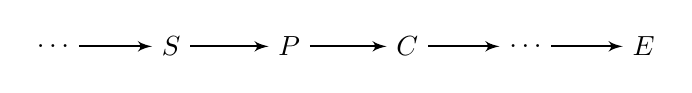
\begin{tikzpicture}[>=latex',node distance = 2.5cm]
\node (S) {$S$};
\node [left of = S, node distance = 1.5cm] (Xo) {$\ldots$};
\draw[->,thick] (Xo) to (S);
\node [right of = S, node distance = 1.5cm] (P) {$P$};
\draw[->,thick] (S) to (P);
\node [right of = P, node distance = 1.5cm] (C) {$C$};
\draw[->,thick] (P) to (C);
\node [right of = C, node distance = 1.5cm] (X1) {$\ldots$};
\draw[->,thick] (C) to (X1);
\node [right of = X1, node distance = 1.5cm] (E) {$E$};
\draw[->,thick] (X1) to (E);
\end{tikzpicture}
\begin{itemize}
\item 1st step
\par
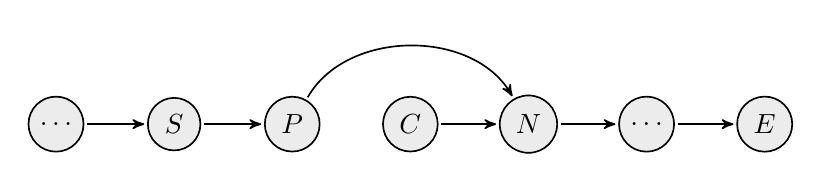
\begin{tikzpicture}[modal]
\node[world] (S){$S$};
\node[world] (X0)[left of = S]{$\ldots$};
\node[world] (P)[right of = S]{$P$};
\node[world] (C)[right of = P]{$C$};
\node[world] (N)[right of = C]{$N$};
\node[world] (X1)[right of = N]{$\ldots$};
\node[world] (E)[right of = X1]{$E$};
\path[->] (X0) edge (S);
\path[->] (S) edge (P);
\path[->] (C) edge (N);
\path[->] (N) edge (X1);
\path[->] (X1) edge (E);
\path[->] (P) edge[bend left=60] (N);
\end{tikzpicture}
\par
\item 2nd step
\par
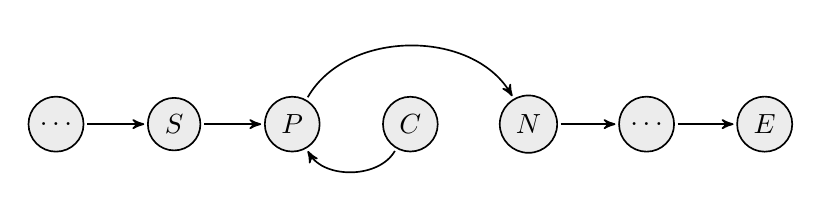
\begin{tikzpicture}[modal]
\node[world] (S){$S$};
\node[world] (X0)[left of = S]{$\ldots$};
\node[world] (P)[right of = S]{$P$};
\node[world] (C)[right of = P]{$C$};
\node[world] (N)[right of = C]{$N$};
\node[world] (X1)[right of = N]{$\ldots$};
\node[world] (E)[right of = X1]{$E$};
\path[->] (X0) edge (S);
\path[->] (S) edge (P);
\path[->] (N) edge (X1);
\path[->] (X1) edge (E);
\path[->] (P) edge[bend left=60] (N);
\path[->] (C) edge[bend left=60] (P);
\end{tikzpicture}
\item 3rd step
\par
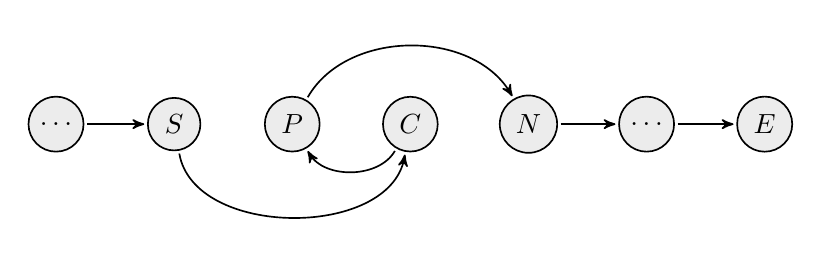
\begin{tikzpicture}[modal]
\node[world] (S){$S$};
\node[world] (X0)[left of = S]{$\ldots$};
\node[world] (P)[right of = S]{$P$};
\node[world] (C)[right of = P]{$C$};
\node[world] (N)[right of = C]{$N$};
\node[world] (X1)[right of = N]{$\ldots$};
\node[world] (E)[right of = X1]{$E$};
\path[->] (X0) edge (S);
\path[->] (N) edge (X1);
\path[->] (X1) edge (E);
\path[->] (P) edge[bend left=60] (N);
\path[->] (C) edge[bend left=60] (P);
\path[->] (S) edge[bend left=280] (C);
\end{tikzpicture}
\item 4th step --- Change $C$ node to $P_{\mathtt{next}}$ i.e. $N$
\par
\begin{tikzpicture}[modal]
\node[world] (S){$S$};
\node[world] (X0)[left of = S]{$\ldots$};
\node[world] (P)[right of = S]{$P$};
\node[world] (D)[right of = P]{};
\node[world] (C)[right of = D]{$C$};
\node[world] (X1)[right of = C]{$\ldots$};
\node[world] (E)[right of = X1]{$E$};
\path[->] (X0) edge (S);
\path[->] (N) edge (X1);
\path[->] (X1) edge (E);
\path[->] (P) edge[bend left=60] (C);
\path[->] (D) edge[bend left=60] (P);
\path[->] (S) edge[bend left=280] (D);
\end{tikzpicture}
\item Then continue from 1st step.
\item At the end of the reverse, $C$ will be at $E$, while $P$ is not moved and $S_{\mathtt{next}}$ is the previous node of $E$, i.e. the final node of this group.
\par
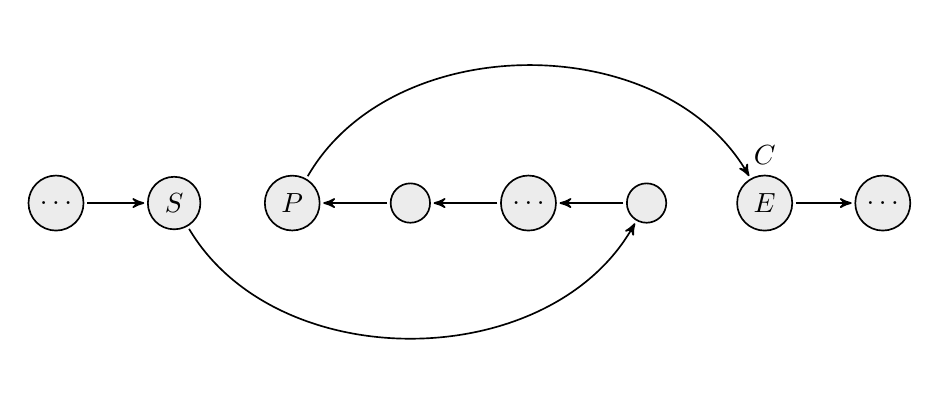
\begin{tikzpicture}[modal]
\node[world] (S){$S$};
\node[world] (X0)[left of = S]{$\ldots$};
\node[world] (P)[right of = S]{$P$};
\node[world] (D1)[right of = P]{};
\node[world] (X1)[right of = D1]{$\ldots$};
\node[world] (D2)[right of = X1]{};
\node[world] (E)[label=above:$C$, right of = D2]{$E$};
\node[world] (X2)[right of = E]{$\ldots$};
\path[->] (X0) edge (S);
\path[->] (P) edge[bend left=60] (E);
\path[->] (D1) edge (P);
\path[->] (X1) edge (D1);
\path[->] (D2) edge (X1);
\path[->] (S) edge[bend left=300] (D2);
\path[->] (E) edge (X2);
\end{tikzpicture}
\item When the reverse function returns, it just return $P$. In the next loop, $P_{next}$ is just the start node of the group.
\end{itemize}

\subsubsection{Algorithm}
\setcounter{algorithm}{0}
\begin{algorithm}[H]
\caption{Reverse link list by $k$ steps}
\begin{algorithmic}[1]
\Statex
\Procedure{ReverseKGroup}{$\mathtt{Head}$, $K$}
\State \textbf{Create} a dummy node $D$.
\State $\mathtt{Prev} := D$ \textbf{and} $D_{\mathtt{next}} = \mathtt{Head}$
\State $\mathtt{Current} := \mathtt{Head}$ \textbf{and} $\mathtt{Count} := 0$
\While{$\mathtt{Current} \neq \mathtt{Null}$}
\State $\mathtt{Count} \gets \mathtt{Count} + 1$
\If{$\mathtt{Count} \bmod K$ = 0}
\State $\mathtt{Prev} \gets \mathtt{Reverse}(\mathtt{Prev}, \mathtt{Current}_{\mathtt{next}})$
\State $\mathtt{Current} \gets \mathtt{Prev}_{\mathtt{next}}$
\EndIf
\EndWhile
\EndProcedure
\Statex
\end{algorithmic}
\end{algorithm}

\begin{algorithm}[H]
\caption{Reverse one segment of link list }
\begin{algorithmic}[1]
\Statex
\Procedure{Reverse}{$\mathtt{Start}$, $\mathtt{End}$}
\State $\mathtt{Prev} := \mathtt{Start}_{\mathtt{next}}$ \Comment $\mathtt{Start} \to \mathtt{Prev}$
\State $\mathtt{Current} := \mathtt{Prev}_{\mathtt{next}}$ \Comment $\mathtt{Start} \to \mathtt{Prev} \to \mathtt{Current}$
\While{$\mathtt{Current} \neq \mathtt{End}$}
\State $\mathtt{Prev}_{\mathtt{next}} \gets \mathtt{Current}_{\mathtt{next}} $
\State $\mathtt{Current}_{\mathtt{next}} \gets \mathtt{Start}_{\mathtt{next}} $ 
\State $\mathtt{Start}_{\mathtt{next}} \gets \mathtt{Current}$ 
\State $\mathtt{Current} \gets \mathtt{Prev}_{\mathtt{next}}$ 
\EndWhile
\EndProcedure
\Statex
\end{algorithmic}
\end{algorithm}

\section{30 --- Substring with Concatenation of All Words}
\textbf{\large{Note:}}
\subsection{Approach: Using Two Hash Maps}
\begin{CJK*}{UTF8}{gbsn}
用一个hash map记录words中每个单词出现的次数,由于题目中已经说明每个单词长度相等,所以,扫描原字符每一个位置,从这个位置用另外一个hash map逐个记录是否含有words中的单词,以及出现的个数是否和已经建立的hash map中对应的单词出现的次数相等,如果超过了,中断搜索继续下个位置,如果这个位置不包含其中的word,也中断搜索。
\par
在下列算法代码中,$M_{C}$是用来记录words中每个单词出现的次数,因为words中的单词可能重复,用$M_{P}$记录扫描输入字符串时记录当前出现的word次数。
\clearpage
\end{CJK*}
\subsubsection{Algorithm}
\setcounter{algorithm}{0}
\begin{algorithm}[H]
\caption{Concatenation of words}
\begin{algorithmic}[1]
\Statex
\Procedure{FindSubString}{$S$, $\mathtt{Words}$}
\State \textbf{Initialize} $M_{C}$ to map word to related count in $\mathtt{Words}$
\State $\mathtt{Result} := \emptyset$
\State $N := \mathtt{Length}(\mathtt{Words})$ \Comment Number of words 
\State $L_W := \mathtt{Length}(\mathtt{Words}[0])$ \Comment length of a single word. All words have same length.
\For{$i \in [0, L_{S} - 1]$}
\State $N_0 := 0$ \Comment Index of word in words
\While{$N_0 < N$}
\State $M_{P} := \emptyset$
\State $S_0 := S[i\ldots N_0\times L_W-1]$ \Comment  Get substr
\If{$S_0 \notin M_{C}$} \Comment $S_0$ is not in words
\State \textbf{Break the \textit{while} loop}
\EndIf
\State $\mathtt{Count}_P \gets M_P[S_0] + 1$ \Comment Get $S_0$ count so far
\State $\mathtt{Count}_C \gets M_C[S_0]$ \Comment Get $S_0$ count from input \textbf{words}
\If{$\mathtt{Count}_P > \mathtt{Count}_C$ }
\State \textbf{Break the \textit{while} loop} \Comment Does not match
\EndIf
\State $N_0 \gets N_0+1$ \Comment Move to next word in input string.
\EndWhile 
\If{$N_0 = N$} \Comment Match all words in input words
\State $\mathtt{Result} \gets \mathtt{Result} \cup i$ \Comment add current index in input string into result.
\EndIf
\EndFor
\EndProcedure
\Statex
\end{algorithmic}
\end{algorithm}
\end{document}
